(i) The bar graph representing the above data is shown in figure \ref{fig:bar39_py}\\
\begin{figure}[!ht]
\centering
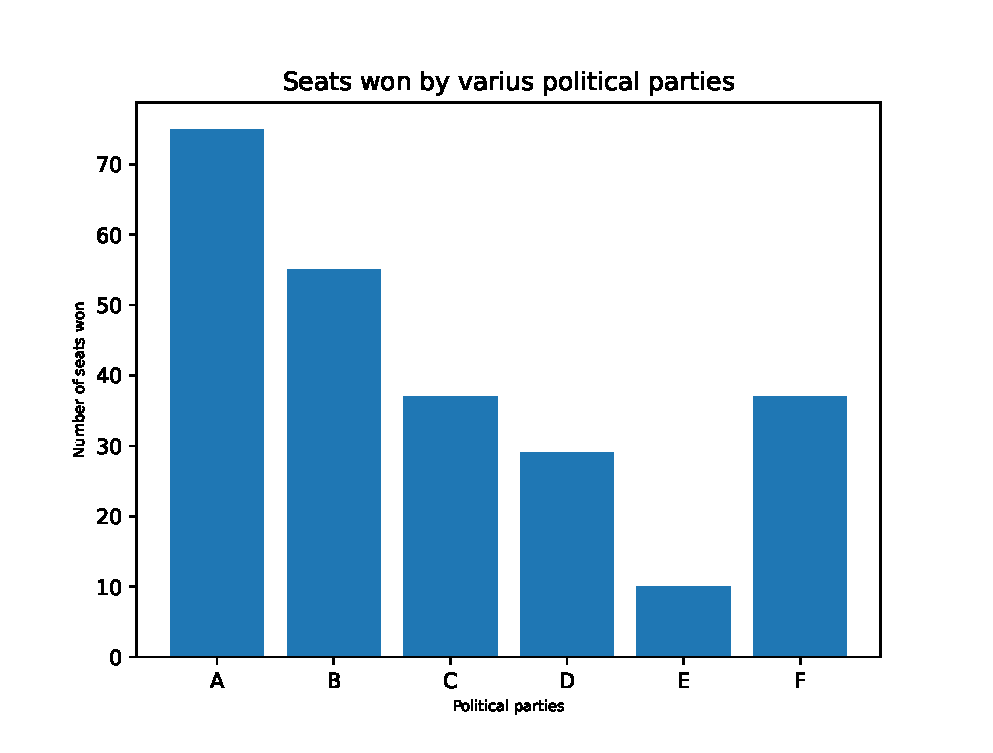
\includegraphics[width=\columnwidth]{./solutions/20-10/stat/codes/pyfigs/exer39.eps}
\caption{Seats won by different political parties}
\label{fig:bar39_py}
\end{figure}
(ii)From the graph in \ref{fig:bar39_py}, Political party A won the maximum seats
The python code used to generate the bar graph for the above problem is
\begin{lstlisting}
./solutions/20-10/stat/codes/exer39.py
\end{lstlisting}
